\chapter{Methods}
\label{chap:methods}
This chapter describes the methods used to carry on the research from the data collection to the results of the analysis. It includes a brief description of the population that took part into the experiment, the experimental task and conditions, the procedure adopted, and the equipment used. Then it delves into the analysis process starting with the preparation and preprocessing of the data and concluding with the intermediate outcomes of the classification. The experiment is the result of a collaboration between the University of Twente, that provided the space, the recruitment system and part of the recording equipment, and myBrainTechnologies that provided their EEG-capable Melomind headsets and the rest of the recording equipment.

\section{Experiment}
\label{sec:experiment}
\subsection{Experimental Annotation app for data collection}
\label{sec:experimental_annotation_app}
An app was developed to collect continuous annotations of perceived emotion, inspired by the design of the FEELTRACE tool \cite{cowie_feeltrace_2000} and the app developed by Thammasan et al. \cite{thammasan_continuous_2016}. The \ac{EA} app was developed in Python using the Psychopy\footnote{https://www.psychopy.org/}  engine for experimental behavioral sciences. The app is a collection of timed routines that alternate guided instructions, emotion annotation tasks on a simplified GUI representing valence-arousal space and forms to report familiarity/liking scores. Three training sessions have been included:
\begin{itemize}
\item T1: the participant is presented with some background information about the valence-arousal model and how to use the annotation tool.
\item T2: the participant is asked to annotate on the \ac{VA} space the perceived emotion while listening to 2 minutes of mixed music genres.
\item T3: the participant is presented with the simulation of a trial of the experiment, including reporting of familiarity/liking and the two listening conditions (see Chapter \ref{sec:task}).
\end{itemize}

The \ac{EA} app was designed and developed at myBrainTechnologies and then tested with the other employees during a short pilot period to adjust the instructions, the clarity of the GUI and the input method. Two input methods were evaluated with A/B testing methodology, using mouse and joystick respectively. The results of the test (see Appendix \ref{app:appendix_A1}) confirmed that using mouse as input source required less training and effort, thus softening the cognitive load of the annotation task while music listening. Using the joystick would have enabled collecting annotation even in an eyes-closed listening condition thanks to the tactile feedback, but at the cost of requiring more training and concentration. To record experimental timed events, the \ac{EA} app was connected to the Melomind through a TriggerBox with an USB cable, a customized Arduino Nano board that can send binary-encoded labels using the serial port. 

\subsection{Participants}
\label{sec:participants}
In respect with the Covid-19 safety measures enforced by University of Twente, 45 healthy participants (28 females) participated in the experiment, all students, or ex-students of the university. The mean age of the population is 23.8 ± 3.1, with the oldest student being 31 years old and the youngest student being 18 years old at the time of the experiment (see Appendix \ref{app:appendix_A2.1}). The lowest educational level was the enrollment as bachelor student and the highest educational level was having completed a master’s degree. Almost half of the participants (20) were Dutch, while all the rest came from different countries, but all of them had at least a C1 or equivalent English proficiency as requirement to enroll in University of Twente. Prior to be confirmed as participants, they were invited through an invitation form informing them on the nature of the experiment and collecting personal information such as demographic information, health conditions, drugs consumption, musical literacy, and some behavioral information on their habits in listening and searching for music to later support the design of a prototype. Almost 5\% of the participants reported to be left-handed, but none asked for an inverted setup of the equipment after it was offered to them (see Appendix \ref{app:appendix_A2.1}). The only strict criterion to participate in the experiment was the capability to hear music, eventually through a hearing support system. None of the applicants was discarded nor required additional support for their health conditions. Prior to their experimental session, they were asked to refrain from consuming recreational drugs and alcohol in the 12 hours before the experiment and caffeine and tobacco in the hour before the experiment to prevent induced biases in the cerebral activity.

\subsection{Stimuli selection}
\label{sec:stimuli}
The stimuli were selected to represent an even as possible distribution of emotions according to the 4 classes identifiable by the quadrants of the Valence-Arousal space. These 4 classes are the possible combinations of positive and negative valence with high and low arousal. To keep consistency with related studies \cite{koelstra_deap_2012}, the classes have been named as follows going clockwise from the top-right quadrant:
\begin{itemize}
\item HAHV: High-Arousal and High-Valence.
\item LAHV: Low-Arousal and High-Valence.
\item LALV: Low-Arousal and Low-Valence.
\item HALV: High-Arousal and Low-Valence.
\end{itemize}
Selecting the right stimuli is a non-trivial task especially in the case of music since many factors can bias the personal perception. For example, familiarity with a certain song might elicit stronger emotions or create an effect of anticipation \cite{sangnark_revealing_2021}, \cite{ward_same_2013}, \cite{salimpoor_anatomically_2011}, while cultural biases or genre preference might completely change how a song is perceived \cite{chang_personalized_2017,fang_perception_2017}. Choosing to include lyrics or no lyrics may shift the attention of the listener from the meaning to the melody and vice versa. It is clearly impossible to address all the possible issues but considering the scope of this study and the research on a realistic use-case scenario, these factors were either mitigated or considered with the due precautions. 

\begin{figure}[h!]
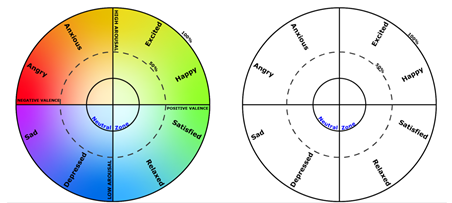
\includegraphics[width=12cm]{img/methods/va_space_experiment.png}
\centering
\caption{The Valence-Arousal space GUI used for the training with color cues on the left, and the uncolored Valence-Arousal space GUI used for the experiment session on the right.} \label{fig_va_space_experiment}
\end{figure}

The stimuli were finally selected as a subset of 8 songs (see Appendix \ref{app:appendix_A2.2}) from the music database created by Koelstra et al. \cite{koelstra_deap_2012}, according to their emotional tagging. Koelstra et al. used the popular online music database last.fm\footnote{https://www.last.fm/}  to retrieve through their APIs 120 songs with associated music videos, emotionally labelled by thousands of users. They then screened them down 40 stimuli during a web assessment session with at least 14 volunteers for each stimulus. The 8 songs selected for this study are a randomly picked subset of those 40 stimuli whose emotional web assessment belonged to the same Valence-Arousal quadrant as the last.fm tagging. For each quadrant there are exactly 2 songs and in total 8 emotions are supposedly portrayed: excitement, happiness, satisfaction, relaxation, depression, sadness, anger, and anxiety. 
It is important to point out that the web assessment conducted by Koelstra et al. was done using the music videos of these songs, and that the placement of the emotions in the \ac{VA} space used in this experiment (see Figure \ref{fig_va_space_experiment}) is just a functional and necessary simplification of the model presented by Russell \cite{russell_circumplex_1980}.

\subsection{Conditions}
\label{sec:conditions}
There is no common agreement in the academic world on which should be the best recording condition for an \ac{EEG} experiment, but most researchers agree on the minimization of external stimuli. Only few studies tried to assess the impact of recording in \ac{EO} condition and \ac{EC} condition on emotion analysis. Barry et al. reported \cite{barry_eeg_2007} differences in topography and power levels, due to the processing of visual input, and recommends considering them when choosing baseline conditions. Chang et al.\cite{chang_experiencing_2015} analyzed recording conditions in relation to music listening and reported that frontal theta power significantly increased in the EC condition, while asymmetries indices in the alpha power on parietal and temporal sites reflected emotional valence for \ac{EC} and \ac{EO} states respectively. In addition, participants rated music as more pleasant and more positive while listening with their eyes closed. These differences in the listening conditions did not seem to significantly impact on the current study that only used frontal electrodes but were considered in the design of the experimental task and in the choice of the resting state baseline. Another problem is caused by ocular movements generates large artifacts in the EEG signal \cite{hagemann_effects_2001}, consequently yielding lower quality data and more computationally expensive preprocessing. In the worst cases, some data must be pruned or reconstructed, varying from a few channels to the entire dataset of a participant. Eye artifacts are typically found in the electrodes placed on the frontal area of the scalp and are usually filtered away by subtracting \ac{EOG} from the \ac{EEG} signal, however it is not the case of this study that could not take advantage of extra sensors to record \ac{EOG} . In general, we can assume that an \ac{EC} condition yields better quality data than an \ac{EO} condition because the quantity of ocular artifacts will be reduced to the minimum and there is no underlying visual stimuli processing. The downsides of experimenting in the \ac{EC} condition are the obvious limitations on the task that could be presented to the participants and a possible increase of power in the Alpha band of the spectrum, that is usually amplified during resting and focused states. The main advantage of the \ac{EO} condition is the possibility to ask the participants for more complex tasks, at the cost of generating more ocular and muscular artifacts and eventually introducing multiple cognitive tasks at once, that can affect the analysis. Prior to the experiment, we run an internal pilot test at myBrainTechnologies to explore the best compromise options between having good quality data, the maximum amount of data and collecting the behavioral data we needed.
Thammasan et al. \cite{thammasan_continuous_2016} opted for a double listening protocol, in \ac{EC} condition to record \ac{EEG} and in \ac{EO} condition to collect affective annotations. This translates into listening twice to the same song but recording only in the \ac{EC} closed condition and then overlapping the annotations taken during the \ac{EO} conditions. Our limitation of 2 frontal electrodes already constrained the collectable amount of data, so we decided to extend this protocol with a double listening and recording approach, in both conditions. During the pilot we explored the feasibility of collecting annotations in both conditions using a joystick, but then opted for collecting annotations only during \ac{EO} condition with a mouse and then reuse the same annotations on the \ac{EEG} data collected in \ac{EC} condition.  As final consideration, the two conditions can be both present in realistic scenarios, with \ac{EO} being the most common listening condition, for example in an office or free-time scenario in which a user listen to music while performing other cognitive tasks (work, homework, gaming…). Listening in \ac{EC} condition resembles a more relaxed scenario, for example when listening to music at the opera or on a comfortable couch in the evening.
